\section{Results}
\label{sec:results}

\subsection{Leakage in the published protocol (H1, H1b)}
\label{sec:leak}
Our rebuild of the authors' own recipe scored
\rqOneCspLdaReplicaPaperReplicaMean\,\% on hand against sixth finger with the
CSP filters fitted on all trials, where the dataset paper reports
85--86\,\%~\cite{wang2026dataset}, and \rqOneCspLdaReplicaCvLeakfreeMean\,\%
with leakage-free cross-validation: we reproduce the direction of the leak,
not the published value. The pre-registered test used our standard CSP+LDA
pipeline (Fig.~\ref{fig:leak}). It reached \rqOneCspLdaPaperReplicaMean\,\%
(95\,\% CI \rqOneCspLdaPaperReplicaCiLo--\rqOneCspLdaPaperReplicaCiHi) with
the filters fitted on all trials and \rqOneCspLdaCvLeakfreeMean\,\%
(\rqOneCspLdaCvLeakfreeCiLo--\rqOneCspLdaCvLeakfreeCiHi) without leakage. The
leak raised every patient's accuracy, by \rqOneHOneDiff{} points on average
(CI \rqOneHOneDiffCiLo--\rqOneHOneDiffCiHi; \rqOneHOneDiffMin{} to
\rqOneHOneDiffMax{} per patient; $W = \rqOneHOneW$, $p = \rqOneHOneP$,
$r = \rqOneHOneR$, $n = \rqOneHOneN$), so H1 is \rqOneHOneCategory.
Leakage-free cross-validation can itself fall below chance when there is
little signal: \rqOneCspLdaCvLeakfreeNBelowChance{} of \rqOneHOneN{} patients
scored under 50\,\% (lowest \rqOneCspLdaCvLeakfreeMin\,\%), and MDM averaged
\rqOneMdmCvLeakfreeMean\,\%. Against the two run-wise splits, which train on
whole runs, the inflation was \rqOneCspLdaPaperReplicaMinusLoroDiff{} points
(leave one run out, CI
\rqOneCspLdaPaperReplicaMinusLoroDiffCiLo--\rqOneCspLdaPaperReplicaMinusLoroDiffCiHi)
and \rqOneCspLdaPaperReplicaMinusChronoDiff{} points (chronological,
\rqOneCspLdaPaperReplicaMinusChronoDiffCiLo--\rqOneCspLdaPaperReplicaMinusChronoDiffCiHi;
both descriptive). TS+LR and MDM, whose steps before the classifier use no
labels, did not change (\rqOneTsLrLeakDiff{} and \rqOneMdmLeakDiff{} points).
The same code inflated healthy-subject accuracy by \rqOneBnciHOneBDiff{}
points on BNCI2014\_001 ($n = \rqOneBnciHOneBN$) and \rqOneChoHOneBDiff{}
points on Cho2017 ($n = \rqOneChoHOneBN$), so H1b is supported: the leak comes
from the procedure, not from these recordings.

Under the run-wise splits, five classical methods separated hand from sixth
finger at only \rqOneHeldOutRunsMeanMin--\rqOneHeldOutRunsMeanMax\,\%, and
sixth finger from rest at
\rqOneSfRestHeldOutRunsMeanMin--\rqOneSfRestHeldOutRunsMeanMax\,\%. Every
result below learns on runs 1--2 and is tested on runs 3--4.

\begin{figure}[t]
  \centering
  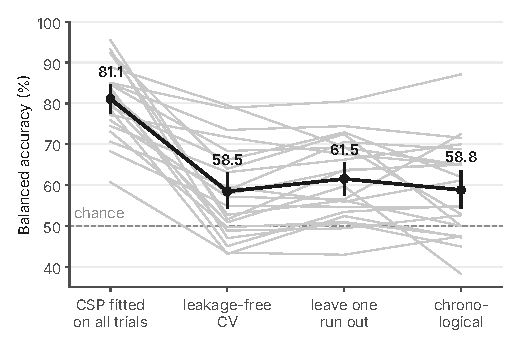
\includegraphics[width=\columnwidth]{figures/paper_leak.pdf}
  \caption{Hand against sixth finger with CSP+LDA, patient by patient
  (pre-therapy session, $n = \rqOneN$): spatial filters fitted on all trials
  before cross-validation, as in the dataset's script; every step fitted
  inside the training folds (leakage-free CV); and the two run-wise splits.
  Grey: patients; black: mean and 95\,\% bootstrap CI; dashed: chance.}
  \label{fig:leak}
\end{figure}

\subsection{Calibration for a new patient (H2a, H2b)}
\label{sec:newuser}
Re-centred transfer with a target weight of \rqTwoHparamRctTslrWeight{} gave
a new patient a fast start and then stayed nearly flat
(Fig.~\ref{fig:setup}). On three classes it reached
\rqTwoRestAhSfRctTslrKOneMean\,\% (CI
\rqTwoRestAhSfRctTslrKOneCiLo--\rqTwoRestAhSfRctTslrKOneCiHi) after one trial
of each movement, and \rqTwoRestAhSfRctTslrKZeroMean\,\% with no labelled
trial, re-centred on the rest periods alone. From scratch, TS+LR reached
\rqTwoRestAhSfTsLrKOneMean\,\%
(\rqTwoRestAhSfTsLrKOneCiLo--\rqTwoRestAhSfTsLrKOneCiHi) from the four windows
of $k = 1$, \rqTwoRestAhSfTsLrKFiveMean\,\% at $k = 5$, and
\rqTwoRestAhSfTsLrKTenMean\,\%, transfer's value after one trial, at $k = 10$.
Transfer stayed near its first value: \rqTwoRestAhSfRctTslrKFiveMean\,\% at
$k = 5$ and \rqTwoRestAhSfRctTslrKAllMean\,\% with the whole pool, where from
scratch reached \rqTwoRestAhSfTsLrKAllMean\,\%. That whole-pool difference,
\rqTwoRestAhSfTsLrMinusRctTslrKAllDiff{} points
(\rqTwoRestAhSfTsLrMinusRctTslrKAllDiffCiLo{} to
\rqTwoRestAhSfTsLrMinusRctTslrKAllDiffCiHi; \rqTwoRestAhSfTsLrMinusRctTslrKAllBetter{}
patients higher from scratch, \rqTwoRestAhSfTsLrMinusRctTslrKAllWorse{} with
transfer), was not tested. Per budget (secondary, Holm), transfer led by
\rqTwoAdvantageKOneDiff{} points at $k = 1$ ($p = \rqTwoAdvantageKOnePHolm$),
\rqTwoAdvantageKFiveDiff{} at $k = 5$ ($p = \rqTwoAdvantageKFivePHolm$) and
\rqTwoAdvantageKTenDiff{} at $k = 10$ ($p = \rqTwoAdvantageKTenPHolm$).

\begin{figure}[t]
  \centering
  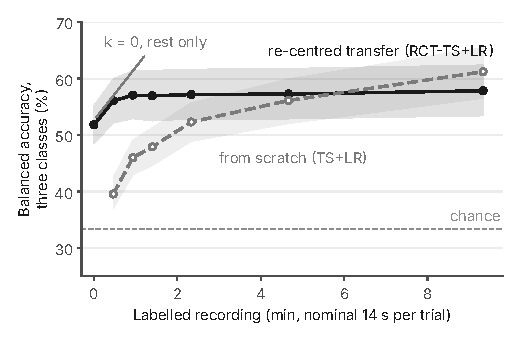
\includegraphics[width=\columnwidth]{figures/paper_calibration.pdf}
  \caption{Calibration for a new patient: three classes, pre-therapy session,
  $n = \rqTwoHTwoAN$. Solid: re-centred transfer from other patients with
  target weight \rqTwoHparamRctTslrWeight{} (RCT-TS+LR); dashed: the same
  classifier from scratch (TS+LR). Points are $k = 0$ (transfer only,
  re-centred on rest), 1, 2, 3, 5, 10 and all trials of each movement, at
  their nominal minutes of labelled recording. Bands are 95\,\% bootstrap CIs.}
  \label{fig:setup}
\end{figure}

The confirmatory tests agree (Table~\ref{tab:tests}). The ALC was larger with
transfer (mean difference \rqTwoHTwoADiff, CI
\rqTwoHTwoADiffCiLo--\rqTwoHTwoADiffCiHi, median \rqTwoHTwoAMedianDiff,
$W = \rqTwoHTwoAW$, $p = \rqTwoHTwoAP$, $r = \rqTwoHTwoAR$), so H2a is
supported. Much of this comes from budgets at which the from-scratch decoder
has very few windows: transfer with no labelled trial already matched from
scratch at $k = 5$. Transfer's lead at $k = 5$ exceeded its lead with the
whole pool by \rqTwoHTwoBPointsDiff{} points ($p = \rqTwoHTwoBP$), so H2b is
supported. Both held without the development patients, with the
chronological draw and on the post-therapy session.

Per patient, \rqTwoReachRestAhSfSixtyBoth{} of the \rqTwoHTwoAN{} reached
60\,\% with both methods, and transfer got there a median of
\rqTwoReachRestAhSfSixtyMedianSaved{} trials per movement sooner;
\rqTwoReachRestAhSfSixtyOnlyScratch{} reached it only from scratch, because
transfer stayed below it, \rqTwoReachRestAhSfSixtyOnlyTransfer{} only with
transfer and \rqTwoReachRestAhSfSixtyNeither{} with neither. At 70\,\%,
\rqTwoReachRestAhSfSeventyBoth{} reached it with both,
\rqTwoReachRestAhSfSeventyOnlyScratch{} only from scratch,
\rqTwoReachRestAhSfSeventyOnlyTransfer{} only with transfer and
\rqTwoReachRestAhSfSeventyNeither{} with neither.
The secondary EEGNet pair also favoured transfer (H2a and H2b supported,
Table~\ref{tab:tests}): the pre-trained network reached
\rqTwoRestAhSfEegnetEaFtKZeroMean\,\% with no labelled trial and
\rqTwoRestAhSfEegnetEaFtKAllMean\,\% with the whole pool, while EEGNet from
scratch rose from \rqTwoRestAhSfEegnetScratchKOneMean\,\% to
\rqTwoRestAhSfEegnetScratchKAllMean\,\%.

\begin{table*}[t]
  \centering
  \caption{Pre-registered tests, pre-therapy session. Effects are mean paired
  differences with 95\,\% bootstrap CIs, in percentage points of balanced
  accuracy, except for H2a and H3, which are on the ALC scale (0 at chance, 1
  perfect). Tests are one-sided for H1, H1b, H2b and H3c and two-sided for H2a
  and H3; $W$ is the positive-rank sum of a one-sided test and the smaller
  rank sum of a two-sided one; $p$ is Holm-adjusted inside two-member
  families ($^\dagger$). Comparisons are transfer minus from scratch unless
  stated; $n = \rqTwoHTwoAN$ patients except on the healthy datasets. The last column repeats the test on the
  post-therapy session ($n = \nPost$; the same categories with
  sub-21 and sub-22 averaged, $n = \rqOneHOnePostLinkedN$).}
  \label{tab:tests}
  \footnotesize
  \setlength{\tabcolsep}{4pt}
  \begin{tabular}{@{}llccccll@{}}
    \toprule
    & Comparison, per patient & Mean difference [95\,\% CI] & $W$ & $r$ & $p$ & Outcome & Post-therapy \\
    \midrule
    H1 & CSP+LDA, hand vs finger: leak minus leakage-free CV & \rqOneHOneDiff{} [\rqOneHOneDiffCiLo, \rqOneHOneDiffCiHi] & \rqOneHOneW & \rqOneHOneR & \rqOneHOneP & \rqOneHOneCategory & \rqOneHOnePostCategory \\
    H1b & The same, BNCI2014\_001 (healthy, $n = \rqOneBnciHOneBN$) & \rqOneBnciHOneBDiff{} [\rqOneBnciHOneBDiffCiLo, \rqOneBnciHOneBDiffCiHi] & \rqOneBnciHOneBW & \rqOneBnciHOneBR & \rqOneBnciHOneBPHolm$^\dagger$ & supported & -- \\
     & The same, Cho2017 (healthy, $n = \rqOneChoHOneBN$) & \rqOneChoHOneBDiff{} [\rqOneChoHOneBDiffCiLo, \rqOneChoHOneBDiffCiHi] & \rqOneChoHOneBW & \rqOneChoHOneBR & \rqOneChoHOneBPHolm$^\dagger$ & supported & -- \\
    H2a & New user, three classes, ALC & \rqTwoHTwoADiff{} [\rqTwoHTwoADiffCiLo, \rqTwoHTwoADiffCiHi] & \rqTwoHTwoAW & \rqTwoHTwoAR & \rqTwoHTwoAP & \rqTwoHTwoACategory & \rqTwoHTwoAPostCategory \\
    H2b & New user: lead at $k = 5$ minus with all & \rqTwoHTwoBPointsDiff{} [\rqTwoHTwoBPointsDiffCiLo, \rqTwoHTwoBPointsDiffCiHi] & \rqTwoHTwoBW & \rqTwoHTwoBR & \rqTwoHTwoBP & \rqTwoHTwoBCategory & \rqTwoHTwoBPostCategory \\
    H3 (a) & New command, finger vs rest, ALC & \rqThreeHThreeADiff{} [\rqThreeHThreeADiffCiLo, \rqThreeHThreeADiffCiHi] & \rqThreeHThreeAW & \rqThreeHThreeAR & \rqThreeHThreeAPHolm$^\dagger$ & \rqThreeHThreeACategory & \rqThreeHThreeAPostCategory \\
    H3 (b) & New command, three classes, ALC & \rqThreeHThreeBDiff{} [\rqThreeHThreeBDiffCiLo, \rqThreeHThreeBDiffCiHi] & \rqThreeHThreeBW & \rqThreeHThreeBR & \rqThreeHThreeBPHolm$^\dagger$ & \rqThreeHThreeBCategory & \rqThreeHThreeBPostCategory \\
    H3c & Finger vs rest, $k = 2$: minus own-hand decoder & \rqThreeHThreeCKTwoPointsDiff{} [\rqThreeHThreeCKTwoPointsDiffCiLo, \rqThreeHThreeCKTwoPointsDiffCiHi] & \rqThreeHThreeCKTwoW & \rqThreeHThreeCKTwoR & \rqThreeHThreeCKTwoPHolm$^\dagger$ & \rqThreeHThreeCKTwoCategory & \rqThreeHThreeCKTwoPostCategory \\
     & The same, $k = 5$ & \rqThreeHThreeCKFivePointsDiff{} [\rqThreeHThreeCKFivePointsDiffCiLo, \rqThreeHThreeCKFivePointsDiffCiHi] & \rqThreeHThreeCKFiveW & \rqThreeHThreeCKFiveR & \rqThreeHThreeCKFivePHolm$^\dagger$ & \rqThreeHThreeCKFiveCategory & \rqThreeHThreeCKFivePostCategory \\
    \midrule
    \multicolumn{8}{@{}l}{\emph{Secondary pair: EEGNet pre-trained and fine-tuned minus EEGNet from scratch}} \\
    H2a & New user, three classes, ALC & \rqTwoEegnetHTwoADiff{} [\rqTwoEegnetHTwoADiffCiLo, \rqTwoEegnetHTwoADiffCiHi] & \rqTwoEegnetHTwoAW & \rqTwoEegnetHTwoAR & \rqTwoEegnetHTwoAP & \rqTwoEegnetHTwoACategory & -- \\
    H2b & New user: lead at $k = 5$ minus with all & \rqTwoEegnetHTwoBPointsDiff{} [\rqTwoEegnetHTwoBPointsDiffCiLo, \rqTwoEegnetHTwoBPointsDiffCiHi] & \rqTwoEegnetHTwoBW & \rqTwoEegnetHTwoBR & \rqTwoEegnetHTwoBP & \rqTwoEegnetHTwoBCategory & -- \\
    H3 (a) & New command, finger vs rest, ALC & \rqThreeEegnetHThreeADiff{} [\rqThreeEegnetHThreeADiffCiLo, \rqThreeEegnetHThreeADiffCiHi] & \rqThreeEegnetHThreeAW & \rqThreeEegnetHThreeAR & \rqThreeEegnetHThreeAPHolm$^\dagger$ & \rqThreeEegnetHThreeACategory & -- \\
    H3 (b) & New command, three classes, ALC & \rqThreeEegnetHThreeBDiff{} [\rqThreeEegnetHThreeBDiffCiLo, \rqThreeEegnetHThreeBDiffCiHi] & \rqThreeEegnetHThreeBW & \rqThreeEegnetHThreeBR & \rqThreeEegnetHThreeBPHolm$^\dagger$ & \rqThreeEegnetHThreeBCategory & -- \\
    \bottomrule
  \end{tabular}
\end{table*}

\subsection{A new command (H3, H3c)}
For the confirmatory pair, transfer showed no clear benefit for the new
command before therapy (Fig.~\ref{fig:rqthree}). Outcome (a), sixth finger
against rest, uses no hand trial (Section~\ref{sec:scenarios}): it is the
detection curve of a newly calibrated command. Transfer reached
\rqThreeSfRestRctTslrKOneMean\,\% with one sixth-finger trial against
\rqThreeSfRestTsLrKOneMean\,\% from scratch, and
\rqThreeSfRestRctTslrKFiveMean\,\% against \rqThreeSfRestTsLrKFiveMean\,\% with
five. The ALC difference favoured transfer, but its CI included zero (median
\rqThreeHThreeAMedianDiff, Holm $p = \rqThreeHThreeAPHolm$), with three
patients far below zero. Outcome (b), three classes, does use
the hand trials. There the from-scratch decoder, trained on unbalanced classes
without class weights, almost never answered ``sixth finger'' (recall
\rqThreeRestAhSfTsLrSfRecallMin--\rqThreeRestAhSfTsLrSfRecallMax\,\% for
$k \leq 5$), while transfer did for \rqThreeRestAhSfRctTslrKFiveSfRecall\,\%
at $k = 5$; still, the ALC difference was small (median
\rqThreeHThreeBMedianDiff, $p = \rqThreeHThreeBPHolm$). H3 is therefore
inconclusive. After therapy outcome (a) was significant (Holm
$p = \rqThreeHThreeAPostPHolm$), so H3 was supported there; its category
differs between sessions, so it did not replicate. The secondary EEGNet pair
favoured transfer on both outcomes (finger against rest: ALC difference
\rqThreeEegnetHThreeADiff, CI
\rqThreeEegnetHThreeADiffCiLo--\rqThreeEegnetHThreeADiffCiHi, Holm
$p = \rqThreeEegnetHThreeAPHolm$), but EEGNet from scratch is weak at these
budgets (\rqThreeSfRestEegnetScratchKOneMean\,\% on finger against rest with
one trial), so this says more about the network than about the command.

\begin{figure}[t]
  \centering
  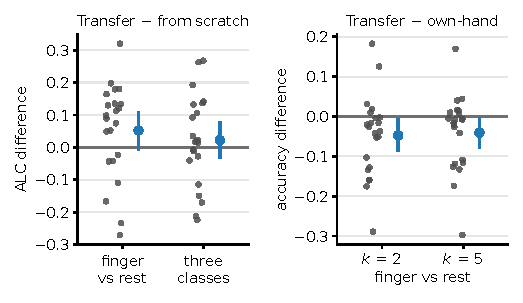
\includegraphics{figures/rq3_patients.pdf}
  \caption{The new command, patient by patient (pre-therapy session,
  $n = \rqThreeHThreeAN$). Left: transfer (RCT-TS+LR) minus from scratch
  (TS+LR), ALC over $k = 1, 2, 3, 5$, for finger against rest (H3a) and three
  classes (H3b). Right: transfer minus the own-hand decoder, finger against
  rest, in points of balanced accuracy (H3c). Grey: patients; black: mean and
  95\,\% CI. Above zero favours transfer.}
  \label{fig:rqthree}
\end{figure}

Whether the sixth finger adds anything to a hand decoder is the question of
the pre-registered own-hand control. A decoder that never saw a sixth-finger
trial detected sixth-finger windows at \rqThreeSfRestAhProxyMean\,\% (CI
\rqThreeSfRestAhProxyCiLo--\rqThreeSfRestAhProxyCiHi), above transfer at
$k = 2$ (\rqThreeSfRestRctTslrKTwoMean\,\%) and $k = 5$
(\rqThreeSfRestRctTslrKFiveMean\,\%). Neither one-sided test was significant
(Holm $p = \rqThreeHThreeCKTwoPHolm$ at both), and both CIs lay below zero
(Table~\ref{tab:tests}): H3c is inconclusive, and the hand decoder did better.
The sixth-finger detectors also called most hand-imagery windows ``sixth
finger'' (own-hand decoder \rqThreeHandAsFingerAhProxy\,\%, transfer
\rqThreeHandAsFingerRctTslrKAll--\rqThreeHandAsFingerRctTslrKOne\,\% for
$k \geq 1$). As pre-registered, we therefore do not claim a distinct
sixth-finger command: its detection may be detection of any imagery.

\subsection{Continuous replay (H4, pre-registered, exploratory)}
H4 expected the sixth-finger command to be detected in most sixth-finger
imagery periods when runs 3--4 were replayed as a continuous signal through
the demonstrator's command gate, as defined before any replay. It was not
met. The three-class decoders trained on the whole pool (CSP+LDA, TS+LR,
RCT-TS+LR and EEGNet from scratch) issued the sixth-finger command in only
\rqFourReplayFingerDetectMin--\rqFourReplayFingerDetectMax\,\% of
sixth-finger periods, with \rqFourReplayFalsePerMinMin--\rqFourReplayFalsePerMinMax{}
false activations per minute of rest and an information transfer rate of
\rqFourReplayItrMin--\rqFourReplayItrMax{} bit/min.

\subsection{Mirrored lesions and other days (exploratory)}
Mirroring the channels of the left-hemiplegic patients, so that every lesion
lay on the same side, did not help transfer: it changed RCT-TS+LR by
\rqFourMirrorRctTslrDiffMin{} to \rqFourMirrorRctTslrDiffMax{} points across
budgets (Holm $p \geq \rqFourMirrorPHolmMin$).

A decoder did not carry over to a later session (Fig.~\ref{fig:later}).
Trained on the first session, TS+LR fell from \rqFourLaterPostWithinPreMean\,\%
within that session to \rqFourLaterPostUnchangedMean\,\% two weeks later
($n = \rqFourLaterPostUnchangedN$), alike after BCI training
(\rqFourLaterPostUnchangedGroupBMean\,\%) and after conventional therapy
(\rqFourLaterPostUnchangedGroupTMean\,\%), and to
\rqFourLaterFollowUnchangedMean\,\% a month after that
($n = \rqFourLaterFollowUnchangedN$). Re-centring it on the new day's rest,
with no labels, recovered part of the loss
(\rqFourLaterPostRecentredKZeroMean\,\% and
\rqFourLaterFollowRecentredKZeroMean\,\%). Five new trials of each movement
added to the old session gave \rqFourLaterPostRecentredKFiveMean\,\% (CI
\rqFourLaterPostRecentredKFiveCiLo--\rqFourLaterPostRecentredKFiveCiHi) and
\rqFourLaterFollowRecentredKFiveMean\,\% when re-centred together, and
\rqFourLaterPostPooledKFiveMean\,\% and \rqFourLaterFollowPooledKFiveMean\,\%
when simply pooled; the five trials alone gave
\rqFourLaterPostNewOnlyKFiveMean\,\% and \rqFourLaterFollowNewOnlyKFiveMean\,\%.
With new trials, re-centring added nothing over pooling; it helped only when
no new trial was recorded.

\begin{figure}[t]
  \centering
  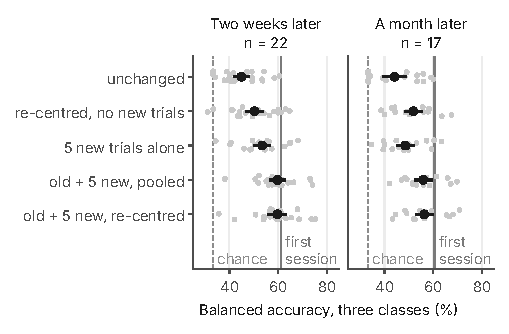
\includegraphics[width=\columnwidth]{figures/paper_later.pdf}
  \caption{The first session's TS+LR decoder on later days (exploratory;
  three classes, runs 3--4): unchanged, re-centred on the new day's rest,
  retrained on five new trials per movement alone, or the old session plus
  five new trials, pooled or re-centred. Grey: patients; black: mean and
  95\,\% CI; solid grey line: the same method within the first session,
  learning on runs 1--2; dashed: chance.}
  \label{fig:later}
\end{figure}

\subsection{The sixth finger as a switch (post hoc)}
\label{sec:switch}
Sixth finger against rest is the contrast these data separate best
(Fig.~\ref{fig:switch}). In a follow-up added after the results, TS+LR on the
14 channels over the movement area separated sixth finger from rest at
\exFourTsLrCentralMean\,\% (CI \exFourTsLrCentralCiLo--\exFourTsLrCentralCiHi),
with \exFourTsLrCentralNAtLeastEighty{} of \rqFourCueN{} patients at 80\,\% or
more. It scored best among the follow-up's candidates on runs 1--2, but its
test score was not unseen: the same configuration had already been scored on
runs 3--4 in the channel-group check below, before the candidates were
listed. Telling hand from sixth finger stayed hard. The best of the decoders
we tried on the test runs, an optimistic best-of-many estimate (the choice on
runs 1--2 agreed), was the pre-trained and fine-tuned EEGNet at
\exFourAhSfEegnetEaFtMean\,\%. The switch turned on for
\exFourTsLrCentralFiresAhMean\,\% of the hand-imagery windows, never seen in
training, against \exFourTsLrCentralFiresSfMean\,\% of sixth-finger and
\exFourTsLrCentralFiresRestMean\,\% of rest windows (sixth finger minus hand
\exFourTsLrCentralFiresSfVsAhDiff{} points, CI
\exFourTsLrCentralFiresSfVsAhDiffCiLo--\exFourTsLrCentralFiresSfVsAhDiffCiHi,
$p = \exFourTsLrCentralFiresSfVsAhP$): it is a switch for imagined movement
more than for the sixth finger.

Window-wise accuracy overstates continuous use. Replayed through the
demonstrator's command gate, the switch turned on in
\exFiveFingerFingerOnMean\,\% of the sixth-finger imagery periods (CI
\exFiveFingerFingerOnCiLo--\exFiveFingerFingerOnCiHi) and
\exFiveFingerHandOnMean\,\% of the hand periods, with
\exFiveFingerFalsePerMinMean{} false activations per minute of rest, and
\exFiveFingerLatencyMean\,s (CI
\exFiveFingerLatencyCiLo--\exFiveFingerLatencyCiHi; mean of the patients'
medians) after the cue of a 6\,s imagery period. A version trained on rest
against any movement caught \exFiveMoveDetectMean\,\% of imagery periods (CI
\exFiveMoveDetectCiLo--\exFiveMoveDetectCiHi) at
\exFiveMoveFalsePerMinMean{} false activations per minute. These comparisons
are uncorrected, and no decoder drove the finger.

Rest was always recorded under a fixation cross and imagery under a picture,
so a channel-group check (post hoc) compared 14
central with five parieto-occipital channels. Sixth finger against rest
decoded better from the central channels (\rqFourCueSfRestCentralMean\,\%
against \rqFourCueSfRestParietoOccipitalMean\,\%). Hand against sixth finger
decoded better from the parieto-occipital ones
(\rqFourCueAhSfParietoOccipitalMean\,\%, CI
\rqFourCueAhSfParietoOccipitalCiLo--\rqFourCueAhSfParietoOccipitalCiHi,
against \rqFourCueAhSfCentralMean\,\%,
\rqFourCueAhSfCentralCiLo--\rqFourCueAhSfCentralCiHi; difference
\rqFourCueAhSfParietoOccipitalVsCentralDiff{} points, CI
\rqFourCueAhSfParietoOccipitalVsCentralDiffCiLo{} to
\rqFourCueAhSfParietoOccipitalVsCentralDiffCiHi,
$p = \rqFourCueAhSfParietoOccipitalVsCentralP$). The weak hand-against-finger
signal may therefore come partly from the two pictures, and after a common
average reference a channel-group contrast cannot separate motor from visual
sources.

\begin{figure}[t]
  \centering
  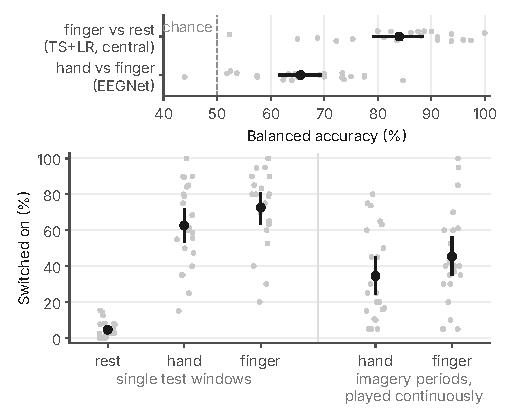
\includegraphics[width=\columnwidth]{figures/paper_switch.pdf}
  \caption{The sixth finger as a switch (post hoc, runs 3--4,
  $n = \rqFourCueN$). Top: sixth finger against rest with TS+LR on the 14
  central channels, and hand against sixth finger with the pre-trained,
  fine-tuned EEGNet. Bottom: how often the switch turns on, for single test
  windows of each kind and, played continuously, for imagery periods. Grey:
  patients; black: mean and 95\,\% bootstrap CI.}
  \label{fig:switch}
\end{figure}
